\documentclass{beamer}
\usepackage{media9}
\usepackage{multimedia}

\usetheme{default}
\title{A Distribution For Magnetic Fields}
\author{Diego Ortiz, UNIR, Wladimir Banda, Hamburg University, \textbf{Federico Zertuche, CENBIO, UTE.}}
\date{\today}

\begin{document}

\begin{frame}
\titlepage
\end{frame}

\begin{frame}{A Distribution For Magnetic Fields}
The team:
\begin{itemize}
  \item[] Diego Ortiz, UNIR (Math).
  \item[] Wladimir Banda, Hamburg University (Physics).
  \item[] Me, UTE (Applied Math).
\end{itemize}
\end{frame}


\begin{frame}{A Distribution For Magnetic Fields}
 \textbf{What we study:}
 \begin{itemize}
  \setlength\itemsep{1em}
  \item[] Role of galactic winds and outflows in galaxy evolution.
  \item[] Remove gas and metals from the disk and nuclear regions of star-forming galaxies and deposit them in the circumgalactic medium.
\end{itemize}
\begin{center}
  \movie[label=show3,width=6cm,height=4cm,poster
  ,autostart,loop]
  {}{movies/video9.mov}
\end{center}
\end{frame}


\begin{frame}{A Distribution For Magnetic Fields}
  \textbf{What we want to understand:}
\begin{itemize}
  \setlength\itemsep{1em}
  \item[] The presence of cold gas (clouds) in such outflows.
\end{itemize}


\textbf{The Wind/Shock - Cloud simulations:}
\begin{itemize}
  \item[] Transport via momentum transfer from hot gas?
  \begin{itemize}
    \item[$\cdot$] In purely hydrodynamic regimes: Too many instabilities, cloud gets destroyed rapidly.
    \item[$\cdot$] Recent simulations show that magnetic stresses can aid cloud acceleration and survival.
  \end{itemize}
\end{itemize}
\end{frame}

\begin{frame}{A Distribution For Magnetic Fields}

  \textbf{In this talk:}
  \begin{itemize}
    \setlength\itemsep{1em}
    \item[$\cdot$] Tools for a systematic statistical study of the effect of magnetic fields.
  \end{itemize}

  \vspace{1em}
  \textbf{Need: Probaility distribution over magnetic fileds.}

  (Herr W.: For magnetic fields with compact support, sometimes symmetric and div-free! And, depending on the day, turbelent too - Kazantsev if dinamos.)

\end{frame}


\begin{frame}{A Distribution For Magnetic Fields}

  \textbf{Need: Probaility distribution over magnetic fileds.}

  \begin{figure}
    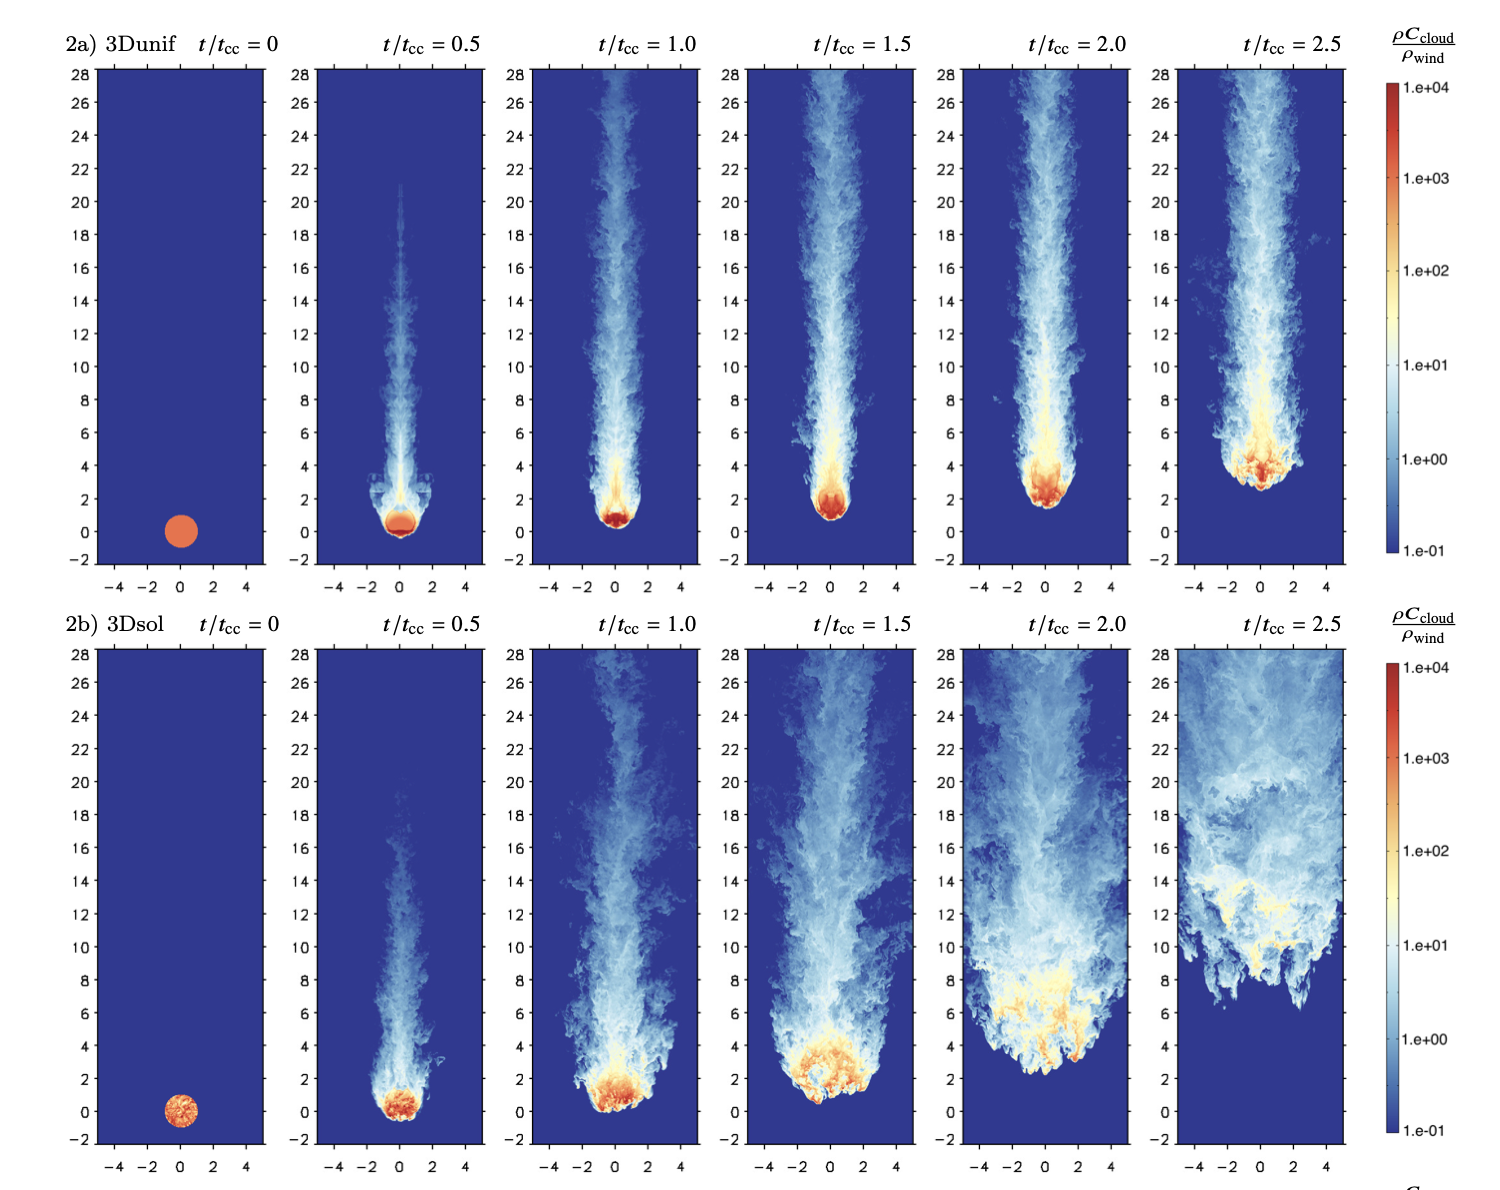
\includegraphics[width=0.85\linewidth]{plots/sample.png}
  \end{figure}

\end{frame}


\begin{frame}{A Distribution For Magnetic Fields}
  \textbf{Need: Probaility distribution over $f: \mathbf{R}^m \rightarrow \mathbf{R}^n$.}

  \textbf{Gaussian Process:} A proba. distribution over a function space.

  \begin{equation*}
    f(x) \sim \mathbf{GP}\left( 0,\ k(x, x')\right)
  \end{equation*}

  For any $\mathbf{x} := [x_1, ... , x_n]^T$,

  \begin{align*}
    \mathbf{f(x)} &\sim
    \mathbf{N}
    \left(
    \begin{bmatrix} 0 \\ \vdots \\ 0 \end{bmatrix}, \
    \begin{bmatrix}
      k(x_1, x_1) \cdots  k(x_1, x_n)\\
      \ddots \\
      k(x_n, x_1) \cdots  k(x_n, x_n)
    \end{bmatrix}
    \right)
  \end{align*}

  where $\mathbf{f(x)} := [f(x_1), ... , f(x_n)]^T$.

\end{frame}


\begin{frame}{A Distribution For Magnetic Fields}

  \textbf{What does that mean?} To simulate:

  \begin{enumerate}
    \setlength\itemsep{1em}
    \item Choose a kernel $k$.
    \item Fix a set of input points $\mathbf{x} := [x_1, ... , x_n]^T$.
    \item To simulate $\mathbf{f(x)}$, build the covariance matrix $\mathbf{K(x, x)}$, draw from $\mathbf{N\left(0, \ K(x, x)\right)}$.
    \vspace{1em}
    \begin{itemize}
      \item[] where $\mathbf{K(x, x)}[i, j] = k(x_i, x_j).$
    \end{itemize}
  \end{enumerate}

\end{frame}


\begin{frame}{A Distribution For Magnetic Fields}

  \textbf{Different covariance functions, different function spaces.}

  \vspace{1em}

  \textbf{Which function space?} You get choose by chossing/building the covariance function $k$.

\end{frame}



\begin{frame}{A Distribution For Magnetic Fields}

  \textbf{Which function space?} Regularity depends on $k$.

  \begin{figure}
    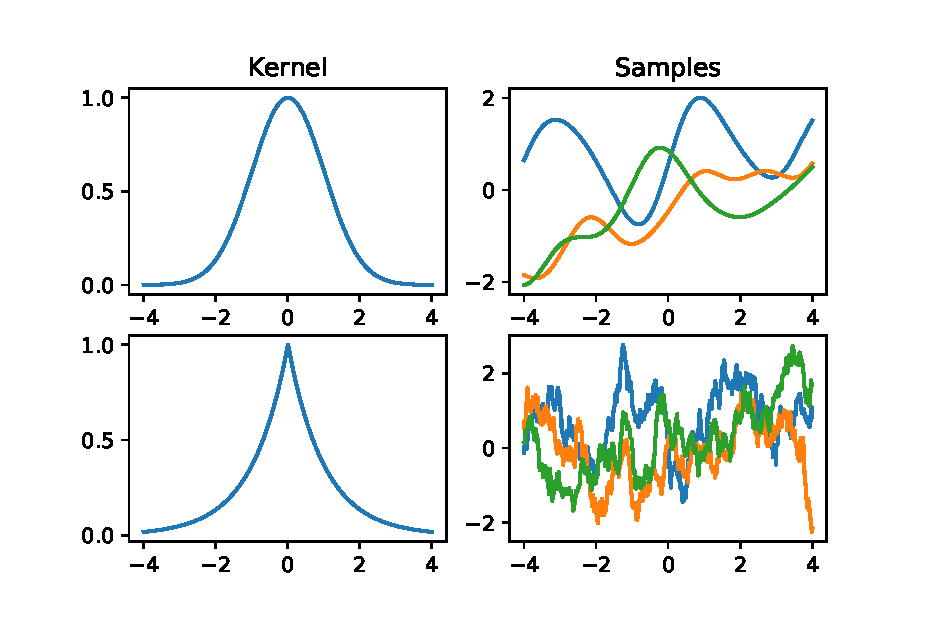
\includegraphics[width=\linewidth]{plots/regularity.eps}
  \end{figure}

\end{frame}


\begin{frame}{A Distribution For Magnetic Fields}

  \textbf{Algebra of covariance functions} Can combine covariance functions to encode other characteristics:

  \vspace{1em}

  \begin{itemize}
    \setlength\itemsep{1em}
    \item[$\cdot$] $\alpha k$ is a covariance function.
    \item[$\cdot$] $k(\phi(x),\ \phi(x'))$ is a covariance function.
    \item[$\cdot$] $k_1 \times k_2$ is a covariance function - like an AND covariance function, high vals if both are.
    \item[$\cdot$] $k_1 + k_2$ is a covariance function - like an OR covariance function, high vals if one is.
  \end{itemize}

\end{frame}


\begin{frame}{A Distribution For Magnetic Fields}

  \textbf{Algebra of covariance functions} Can combine covariance functions to encode other characteristics: $k_1 \times k_2$

  \begin{figure}
    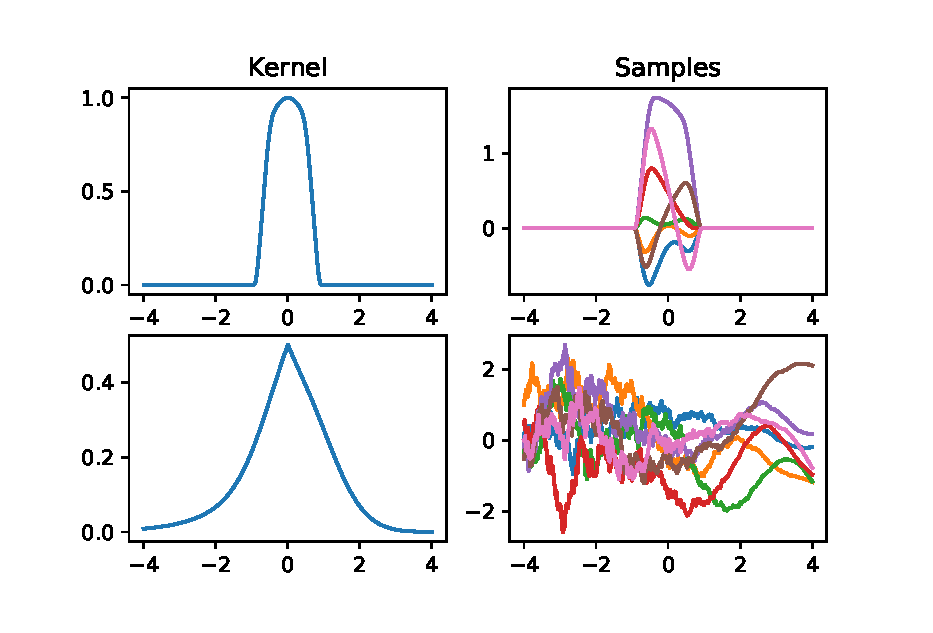
\includegraphics[width=\linewidth]{plots/multiply.eps}
  \end{figure}

\end{frame}


\begin{frame}{A Distribution For Magnetic Fields}

  \textbf{Algebra of covariance functions} Can combine covariance functions to encode other characteristics: $k_1 + k_2$

  \begin{figure}
    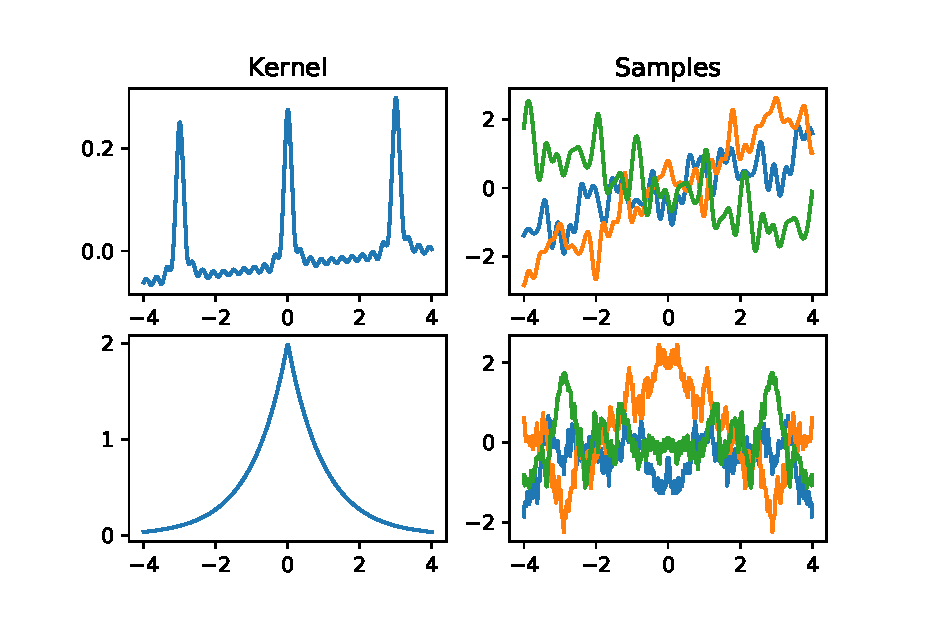
\includegraphics[width=\linewidth]{plots/sum.eps}
  \end{figure}

\end{frame}


\begin{frame}{A Distribution For Magnetic Fields}

  \textbf{A process $R \rightarrow R^2$} Is a distribution over doodles.
  \begin{figure}
    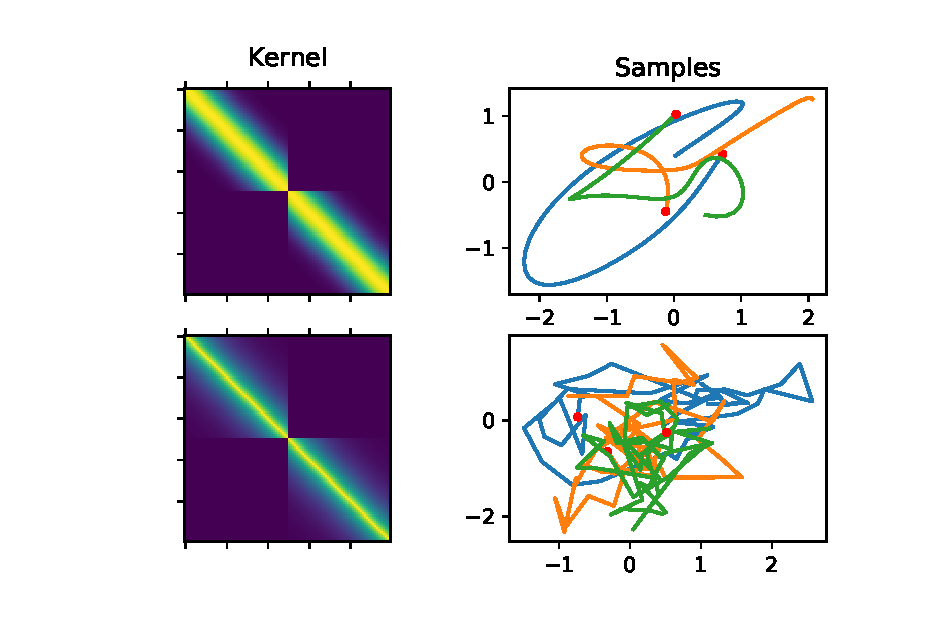
\includegraphics[width=\linewidth]{plots/parametric_curves.eps}
  \end{figure}

\end{frame}


\begin{frame}{A Distribution For Magnetic Fields}

  \textbf{A process $R^2 \rightarrow R^2$} Is a distribution over vector fields.
  \begin{figure}
    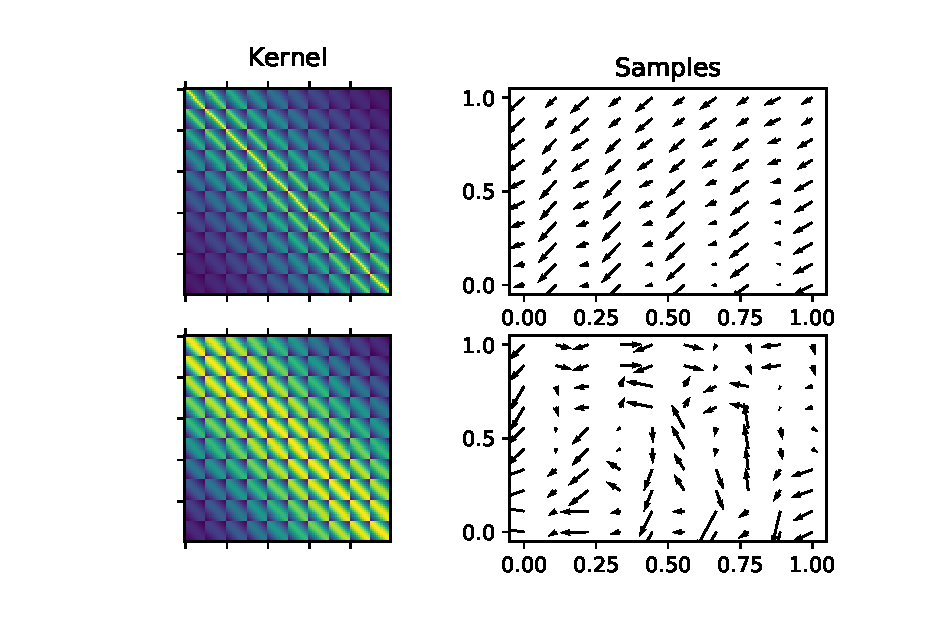
\includegraphics[width=\linewidth]{plots/vector_fields.eps}
  \end{figure}

\end{frame}


\begin{frame}{A Distribution For Magnetic Fields}

  In fact you can encode more:

  \vspace{1em}

  \textbf{Div-Free}:

  \begin{equation*}
    \nabla f = 0
  \end{equation*}

  i.e. Processes that satisfy a linear contraint.

  \begin{equation}\label{eq:linCond}
    \mathcal{L}f = 0
  \end{equation}

  (Idea: Find an operator $\mathcal{G}$ such that $\mathcal{L}\mathcal{G} = 0$. Then, $\mathcal{G}f$ satisfies (\ref{eq:linCond}).)
\end{frame}

\begin{frame}{A Distribution For Magnetic Fields}

  \textbf{Div-Free}: Samples from a div-free \textbf{GP}.

  \begin{figure}
    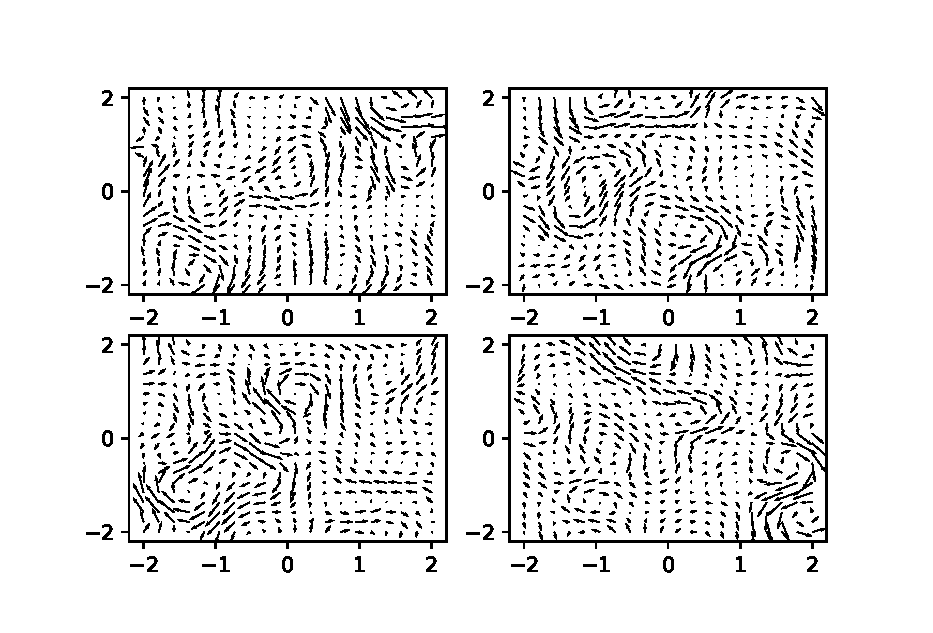
\includegraphics[width=\linewidth]{plots/div_free.eps}
  \end{figure}

\end{frame}

\begin{frame}{A Distribution For Magnetic Fields}

  \textbf{MHD simulation}:

  \begin{center}
    \movie[label=show3,width=10cm,height=8cm,poster
    ,autostart,loop]
    {}{movies/MHD_sim.mov}
  \end{center}

\end{frame}

\begin{frame}{A Distribution For Magnetic Fields}

  \textbf{Curl-Free}: Samples from a curl-free \textbf{GP}.

  \begin{figure}
    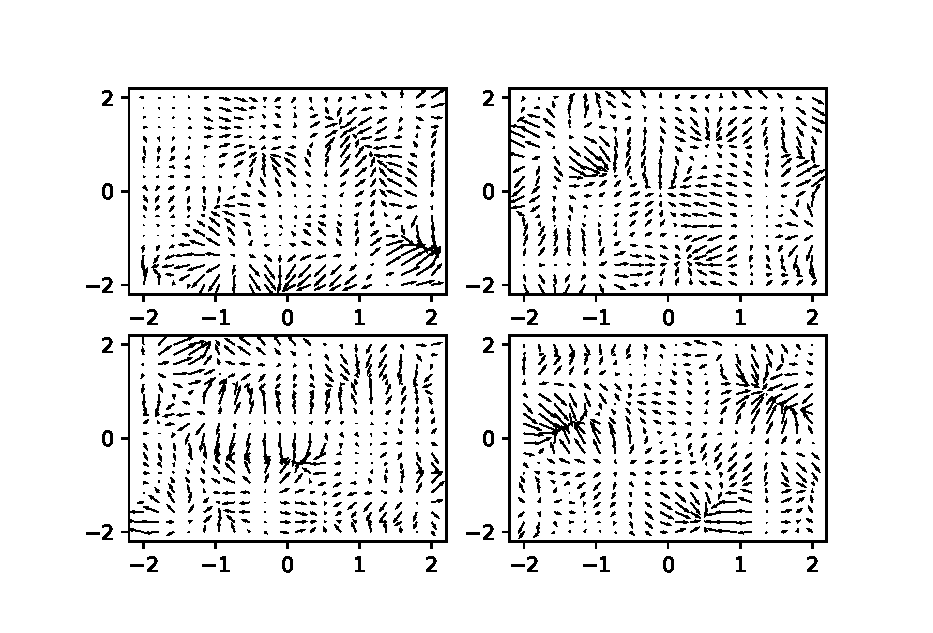
\includegraphics[width=\linewidth]{plots/curl_free.eps}
  \end{figure}

\end{frame}


\begin{frame}{A Distribution For Magnetic Fields}

  \textbf{Trubulence and Kernels:}

  \begin{figure}
    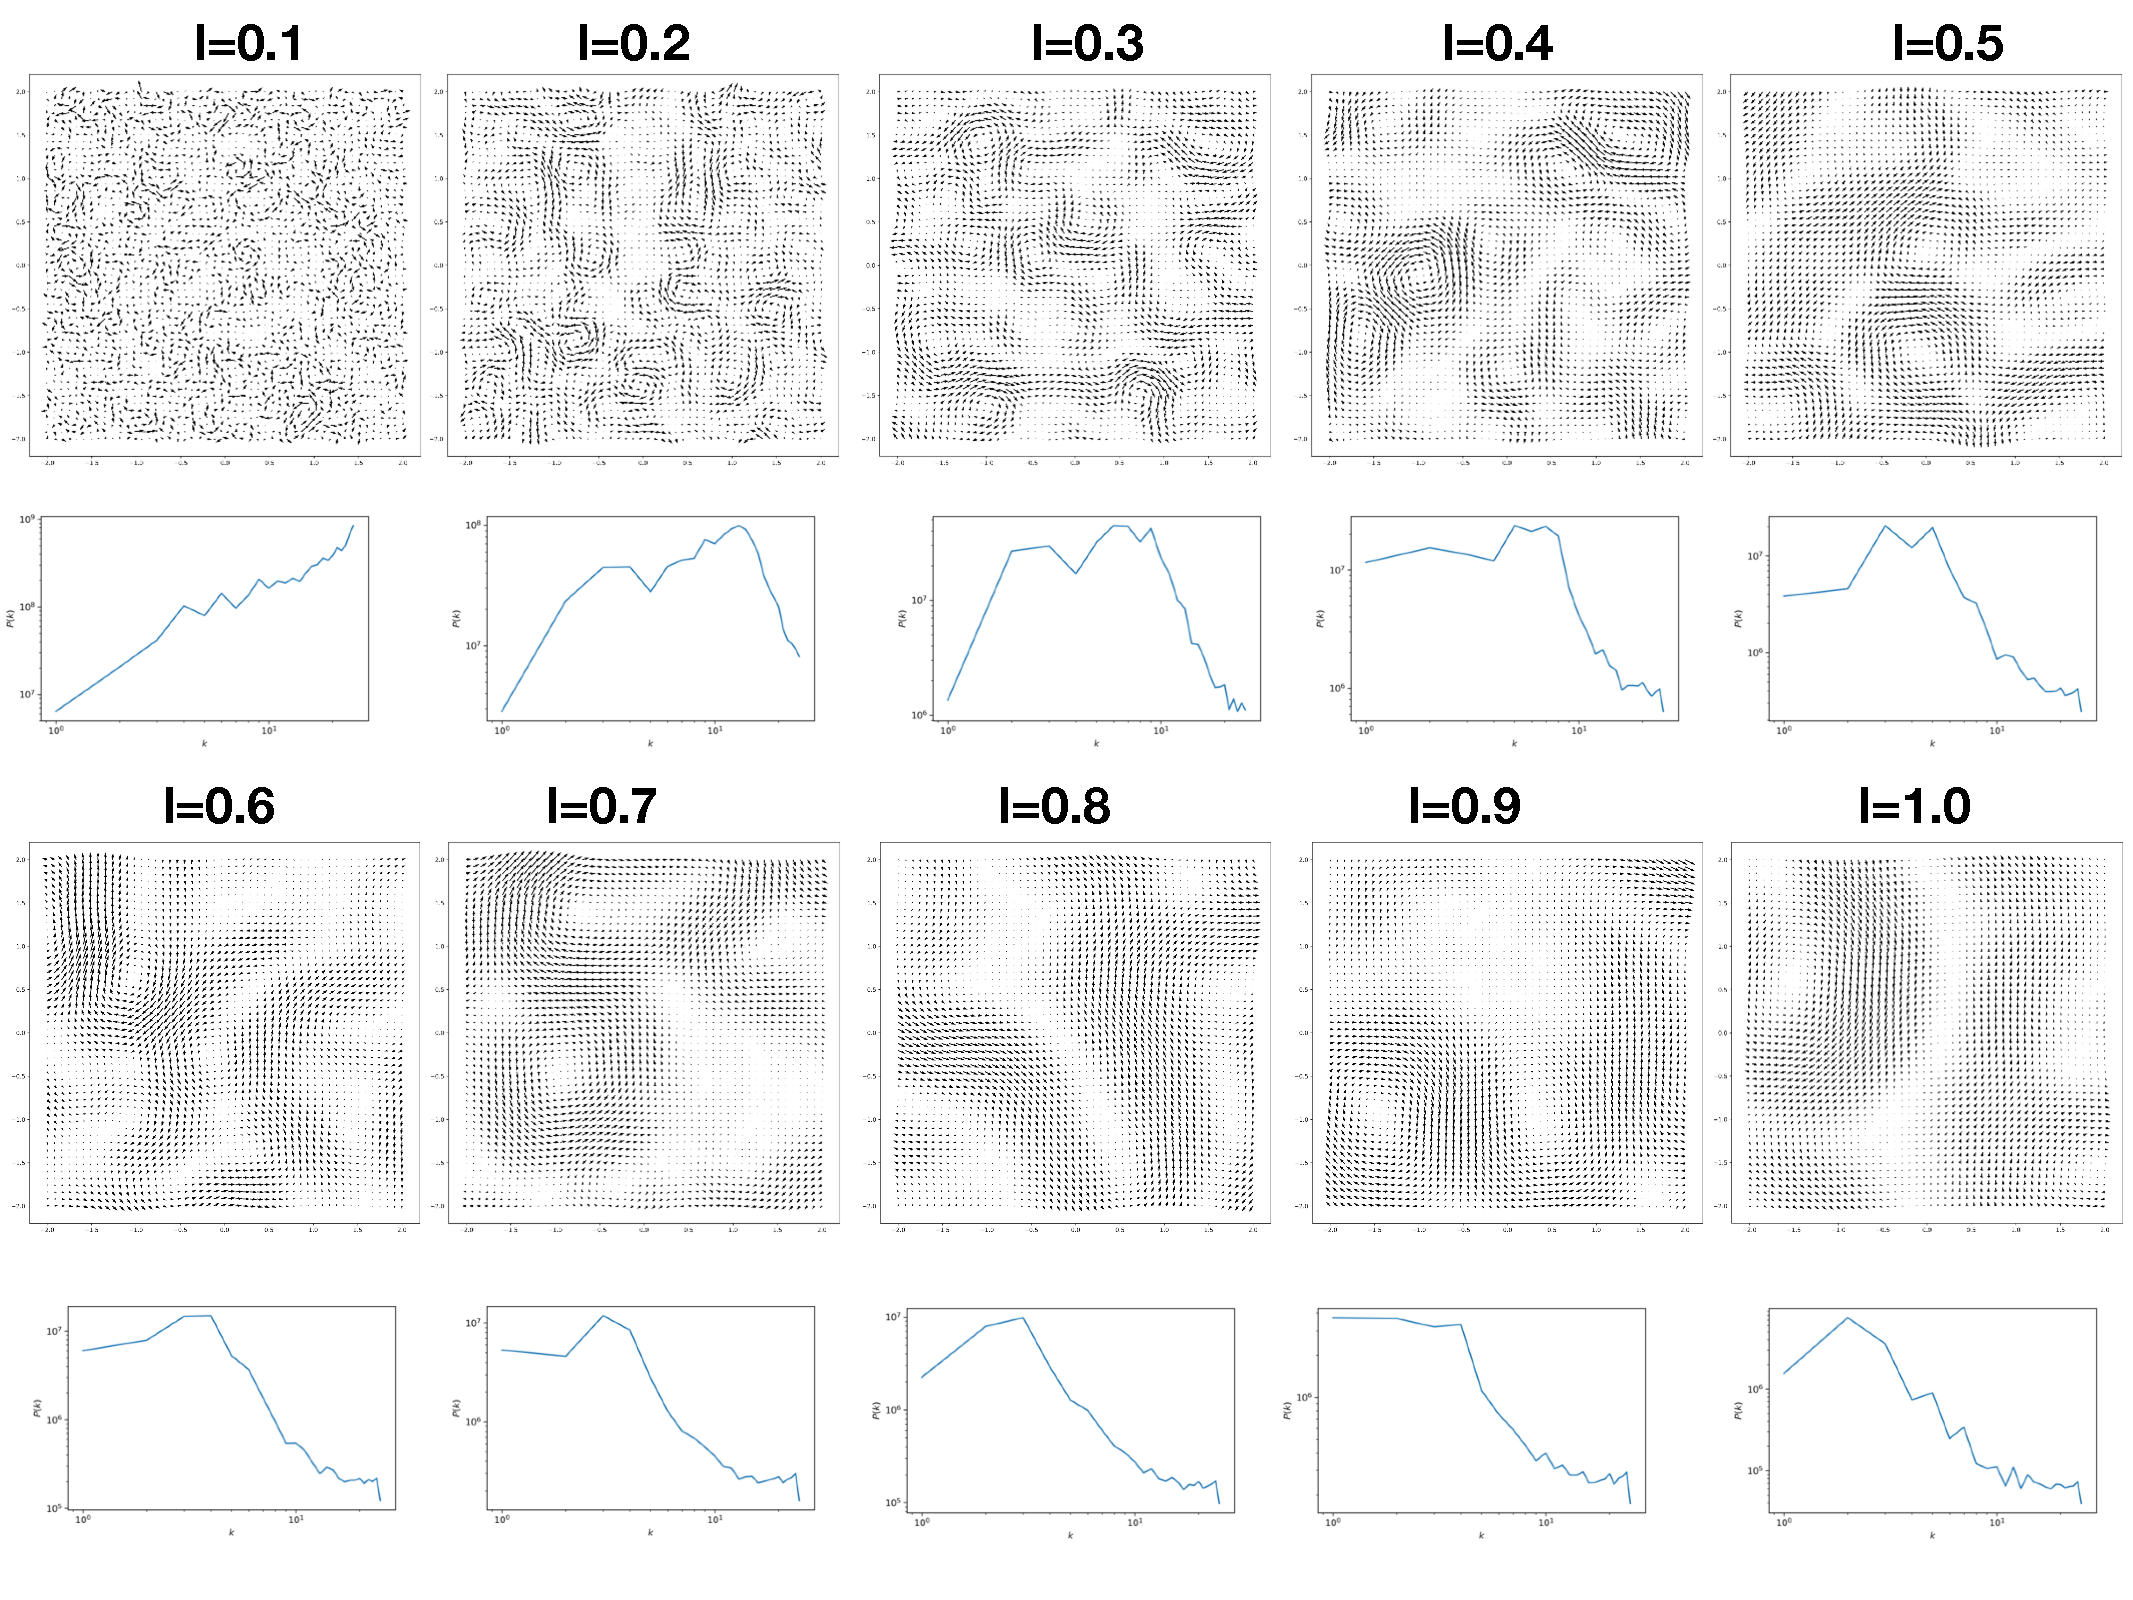
\includegraphics[width=0.9\linewidth]{plots/Power_Spectra.pdf}
  \end{figure}

\end{frame}


\begin{frame}{A Distribution For Magnetic Fields}

  \textbf{So far:}
  \begin{itemize}
    \item[$\cdot$] Distributions over function spaces.
    \item[$\cdot$] Mathematically Expressive: Can encode regularity, symmetries, changes, support.
  \end{itemize}

  \textbf{In progress:}
  \begin{itemize}
    \item[$\cdot$] Computationally NOT Expressive: Autodiff code in progress.
    \item[$\cdot$] Turbulence NOT clear: Studying the relationship between kernels and energy spectral decay.
  \end{itemize}

\end{frame}

\begin{frame}{A Distribution For Magnetic Fields}

  \textbf{A bigger picture:}
  \begin{figure}
    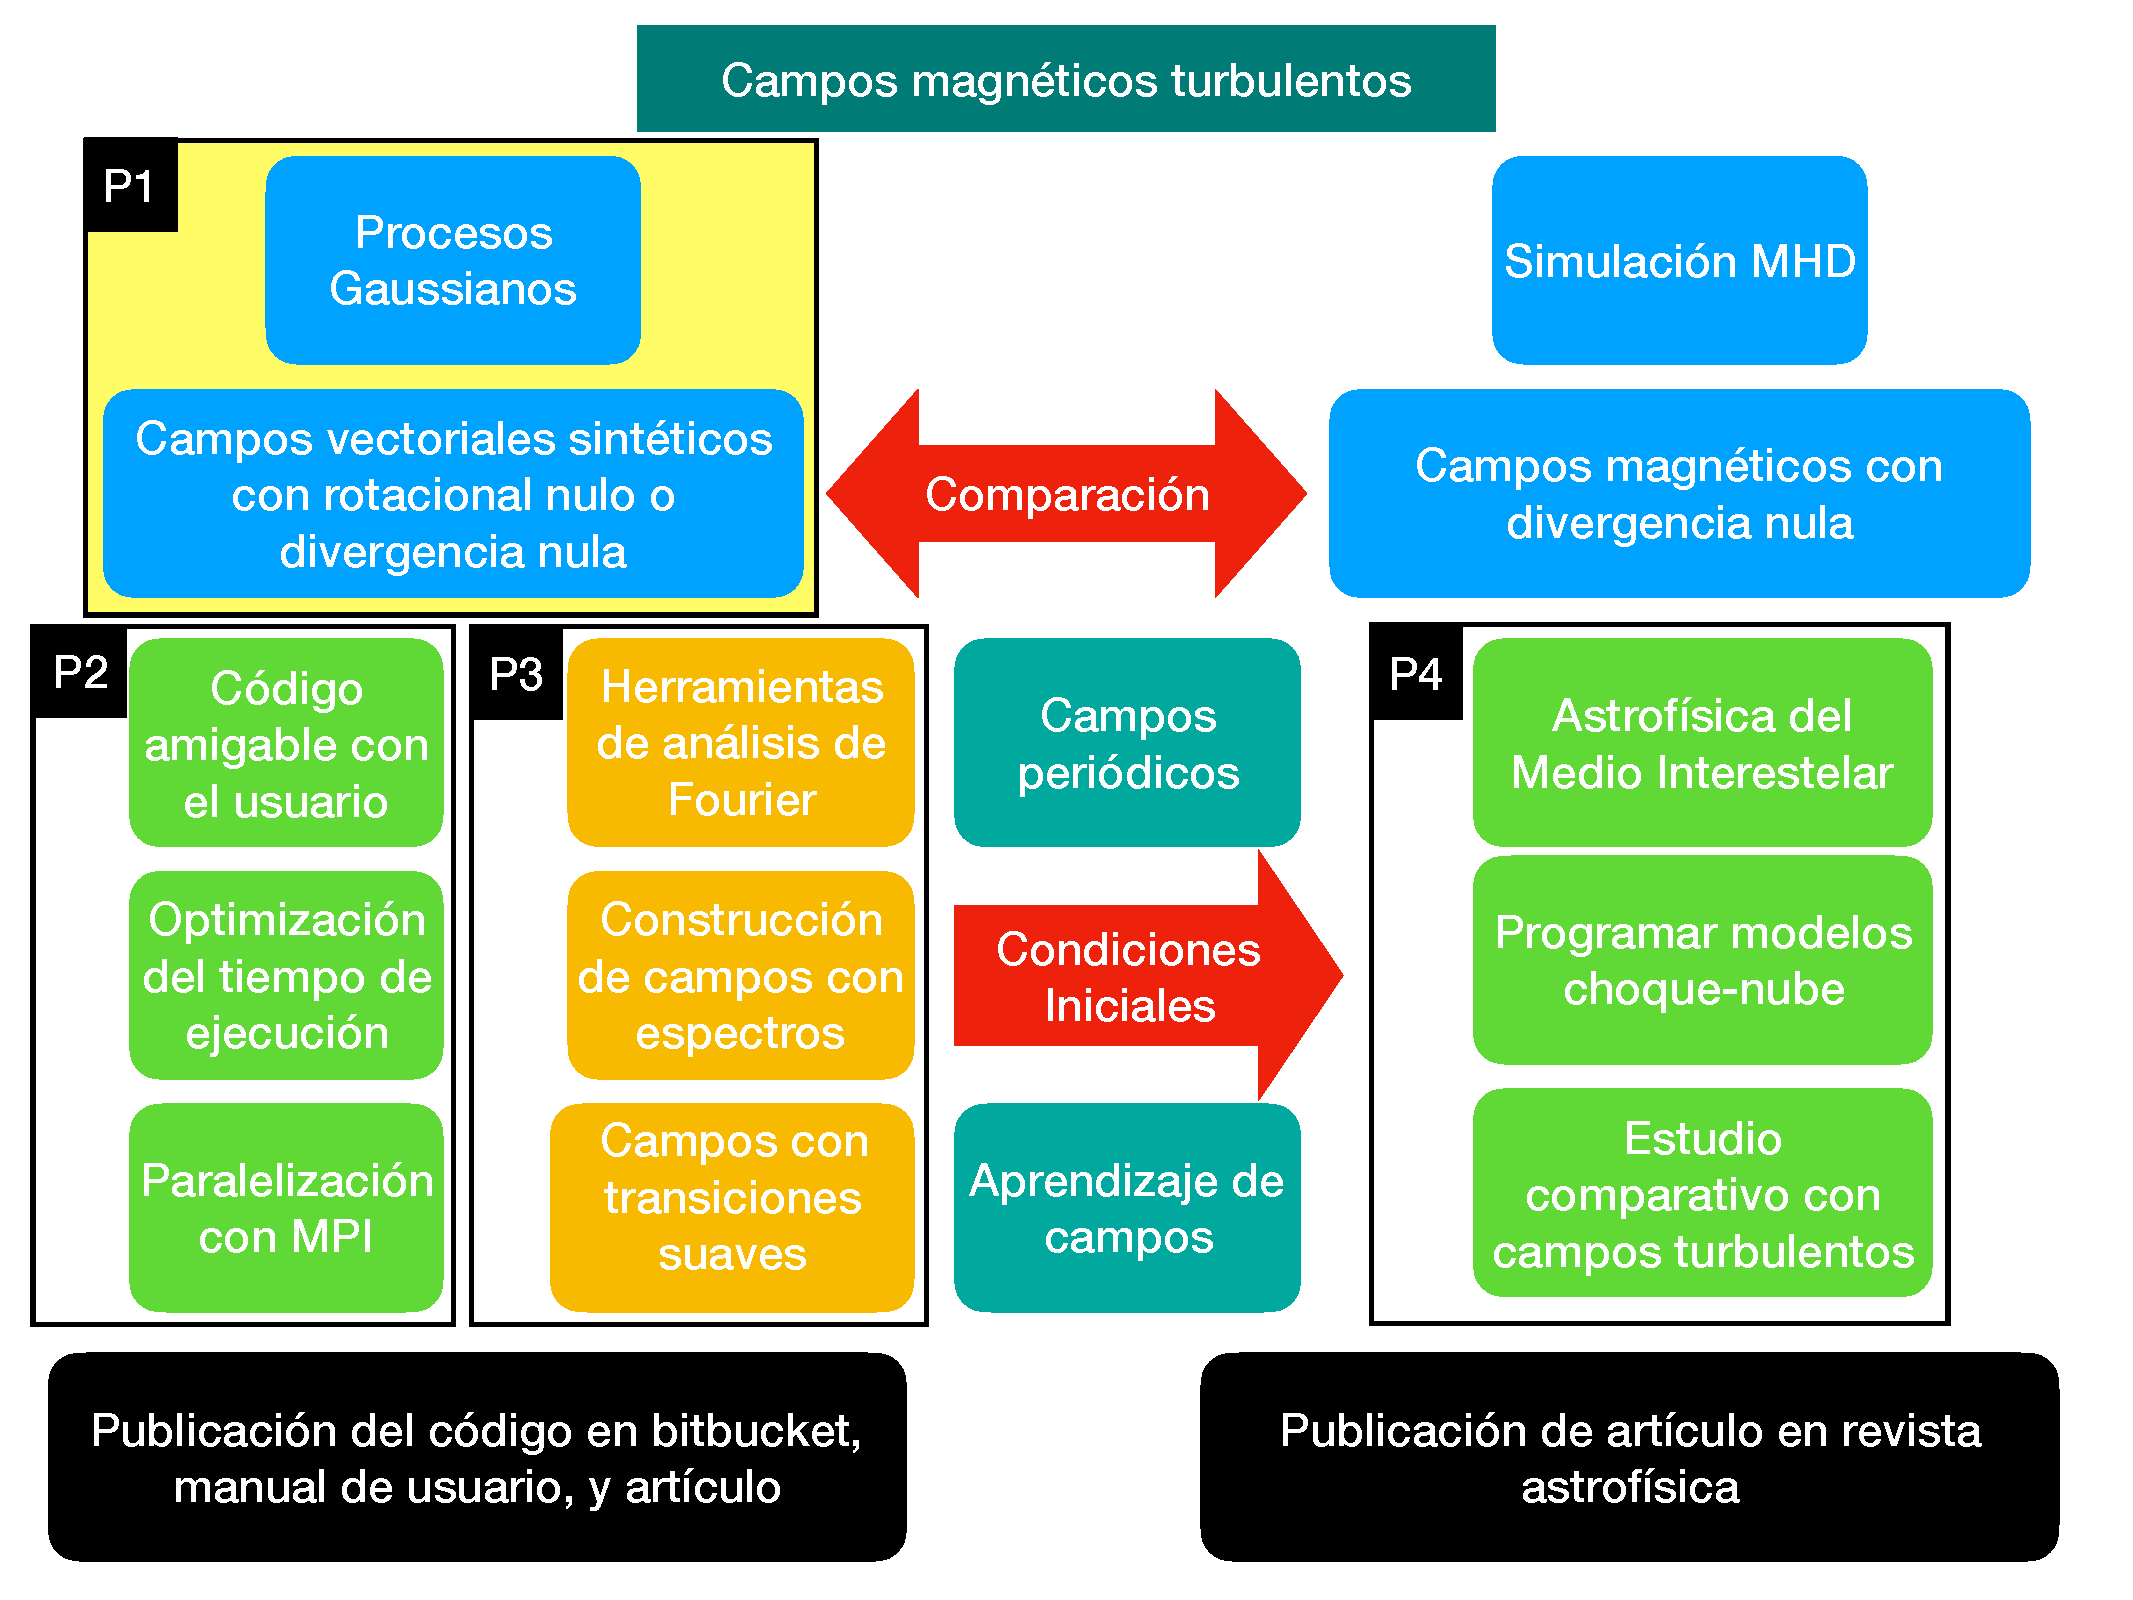
\includegraphics[width=\linewidth]{plots/Sub-proyectos.pdf}
  \end{figure}

\end{frame}

\begin{frame}{A Distribution For Magnetic Fields}

  \textbf{A bigger picture:} (In alphabetical order)

  \vspace{1em}

  \begin{itemize}
    \item[$\cdot$] Computer Science, Math, Physics.
    \item[$\cdot$] Australia, Ecuador, Germany.
  \end{itemize}
\end{frame}


\begin{frame}{A Distribution For Magnetic Fields}

  \textbf{Some refferences:}

  \vspace{1em}

  \begin{itemize}
    \item[$\cdot$] D. Ortiz (2019). \emph{Procesos Gaussianos aplicados al estudio de gases magnetizados.} Msc Thesis.
    \item[$\cdot$] W. E. Banda-Barraga, F. J. Zertuche, C. Federrath, J. Garcıa Del Valle, M. Bruggen, and A. Y .Wagner (2019). \emph{On the dynamics and survival of fractal clouds in galactic winds.} MNRAS.
    \item[$\cdot$] D. Maclaurin. \emph{Modeling, Inference and Optimization with Composable Differentiable Procedures}, PhD. Thesis. https://dougalmaclaurin.com/phd-thesis.pdf
  \end{itemize}
\end{frame}

\end{document}
